\chapter{Návrh vizualizácie}
Wolfgang Aigner vo svojej knihe \textit{Visualization of Time-Oriented Data} \cite{TimeOrientedData} tvrdí, že riešenie problému vizualizácie vyžaduje zodpovedanie troch otázok: 
\begin{easylist}
	# Čo je vizualizované? - Čas a dáta
	# Prečo je to vizualizované? - Požiadavky používateľov
	# Ako je to vizualizované? - Vizuálna reprezentácia \\
\end{easylist}
\noindent Táto kapitola by mala odpovedať na všetky tieto tri položené otázky. 

\section{Charakteristika dát}
V prvom rade nám do verifikácie vstupujú surové dáta, ktorými sú pozorovania a predpovede. Pri porovnávaní týchto dvoch dátových množín sme sa rozhodli, že ich zredukujeme na jednu množinu reprezentujúcu objektívne porovnanie predpovedí a pozorovaní so zachovaním nie všetkej, ale iba dôležitej- informácie. Touto dátovou množinou je teda množina chýb predpovedí, ktorú vytvoríme tak, ako je opísané v podsekcii \ref{subsec:pairing} a sekcii \ref{sec:errormeasurement}.

Výsledkom tohto procesu je tabuľka chýb, kde je pre každý dátum predpovede $ n $ hodín predpovedaných hodnôt, v našom prípade 48, keďže išlo o dvojdňové predpovede. Tieto dáta v systéme ďalej spracúvame. V prvom rade ich rozdelíme na časové podintervaly na základe konfigurácie, defaultne na mesiace. Následne sa pre každý podinterval a každú hodinu predpovede vypočítajú štatistiky opísané v sekcii \ref{sec:errormeasurement}. Takýmto predspracovaním sme získali dva druhy dát v podobnom ale trocha rozdielnom formáte. Ako sme spomenuli, hodnoty chýb sú v tabuľke pre každý dátum predpovede, hodnoty štatistík sú však pre časový interval predpovedí, nie len jeden konkrétny dátum.

V terminológii vizualizácie informácií hovoríme o numerických, ordinálnych a spojitých dátach, no v prvom rade ide o časovo orientované dáta. Pri tomto druhu dát je rozhodujúcou zložkou čas, ktorý opíšeme pomocou stručných charakteristík na základe už spomenutej knihy \textit{Visualization of Time-Oriented Data} \cite{TimeOrientedData}. \\
Pri čase skúmame tieto charakteristiky\footnote{V zátvorke za charakteristikou sa nachádzajú možnosti delenia času na základe tejto charakteristiky. Hrubým písmom je zvýraznená vlastnosť pre naše dáta.}: 

\begin{itemize}
	\item \textit{Škála} (ordinálna/\textbf{diskrétna}/spojitá): Aj z pohľadu predpovedí aj z pohľadu predpovedaných hodín ide o diskrétnu škálu, keďže predpovede sú v diskrétnych časových bodoch, medzi ktorými neuvažujeme nejaké ďalšie body.
	\item \textit{Rámec} (\textbf{bodový}/\textbf{intervalový}): Spomenuli sme, že hodnoty štatistík sú pre časový interval, preto je časový rámec intervalový. Časový rámec pre zvyšné dáta je však bodový, teda bezrozmerný okamih v čase. 
	\item \textit{Usporiadanie} (\textbf{lineárne}/cyklické): Dáta nás môžu navádzať k tomu, aby sme vnímali čas aj ako cyklický, keďže máme neustále opakujúce sa elementy, teda naše dvojdňové predpovede. Časové usporiadanie je však lineárne, keďže čas predpovede je úplne iný čas predpovedných hodín.
	\item \textit{Nahliadanie} (\textbf{usporiadané}/vetvené/mnoho perspektív): Časové udalosti sa nijako nevetvia, ani nemáme dva pohľady na čas, preto ide o jednoducho usporiadaný čas.
	\item \textit{Zrnitosť} (žiadna/\textbf{single}/multi): Čas pre nás je rozdelený na časové jednotky, ktoré však ani nespájame, ani nerozdeľujeme na menšie. Preto hovoríme o granularite, teda zrnitosti, ale iba o single a nie multi.
	\item \textit{Časové primitívi} (\textbf{okamih}/interval/obdobie): Napriek tomu, že rámec je bodový aj intervalový, jedinou časovou primitívou je okamih. Dôvodom je to, že pre každý interval v tabuľke máme vždy iba jedinú hodnotu a nechápeme ho ako \textit{interval} (v zmysle časovej primitívi), ale ako \textit{okamih}.
	\item \textit{Determinovanosť} (\textbf{determinovaný}/nedeterminovaný): Naše dáta neposkytujú žiadnu časovú nejednoznačnosť, preto sa zjavne jedná o determinovaný čas.
\end{itemize}

Autor v knihe ďalej spomína opisné charakteristiky pre časovo orientované dáta, ktoré sú tieto štyri: \textit{škála}, \textit{referenčný rámec}, \textit{druh dát}, \textit{počet premenných}. V stručnosti to zhrnieme tak, že naše dáta sú kvantitatívneho charakteru, abstraktné, určujúce stavy a nie udalosti s mnohými premennými. Všetky tieto charakteristiky priamo vplývajú na návrh vizualizácie. 

\section{Špecifikácia požiadaviek na vizualizáciu}
V tejto sekcii sa snažíme stručne zhrnúť hlavné požiadavky na vizualizáciu vyššie spomenutých dát. V prvom rade, by sme chceli zachovať základné požiadavky kladené na dobrý návrh vizualizácie vo všeobecnosti a neskôr skonkretizovať naše požiadavky pomocou \textit{užívateľských úloh}.

\subsection{Tri základné požiadavky}
Dobrý dizajn vizualizácie sa, tak ako v iných odvetviach, snaží dosiahnuť fungujúcu rovnováhu medzi troma zložkami: \textit{utilitas}, \textit{firmitas}, \textit{venustas} \cite{XYZ}, čo sa z latinčiny dá voľne preložiť ako \textit{užitočnosť}, \textit{robustnosť}, \textit{atraktivita}. Keďže sa v našom prípade jedná o odbornú vizualizáciu, tak sa budeme hlavne sústrediť na prvé dve požiadavky \textit{užitočnosť}, \textit{robustnosť}.
	
\paragraph{\textit{Užitočnosť}} zahŕňa funkcionalitu, funkčnosť, použiteľnosť a podobné pojmy. Vo vizualizácii sú tieto aspekty zhrnuté dvoma mierami - \textit{efektnosť} (presnosť a úplnosť informácie, ktorú chcel užívateľ získať) a \textit{efektivita} (množstvo zdrojov - zvyčajne času - potrebných na získanie žiadanej informácie). Našou úlohou pri návrhu optimálnej vizualizácie je teda pokúsiť sa, aby bola v čo najväčšej miere efektná a efektívna. 

Toto sa pokúsime dosiahnuť rôznymi prostriedkami. 
- \textit{focus+context} \\
- vyuzitie tohto, co meteorologovia uz poznaju \\


\paragraph{\textit{Robustnosť}} je pojem hovoriaci o odolnosti vizualizácie voči chybným, veľkým, rôznorodým dátam. To znamená, že ako dobre a akým spôsobom sa vysporadúva s týmito problémami. Taktiež hovorí o správnosti vizualizácie, teda či berie do úvahy ľudský percepčný systém a nejakým spôsobom nedodáva klamlivú informáciu. Hovoríme o javoch, ktoré poznáme zvyčajne z optických ilúzií. Príkladom môže byť vnímanie perspektívy, kontextuálne vnímanie farieb, vnímanie hodnôt na základe plochy a nie dĺžky a iné podobné javy, na ktoré je nutné dávať pozor.


\paragraph{\textit{Atraktivita}} alebo tiež estetika - krása daného riešenia. Tento pojem nie je limitovaný vizuálnou stránkou vizualizácie, ale taktiež nejasným aspektom, akými sú originalita, inovácia a novosť. Článok od Moera a Purchaseho \cite{RoleOfDesign} tvrdí, že tento aspekt je priveľmi podceňovaný, no i my sa radíme medzi- tých, ktorí nekladú naň taký dôraz, ako na predošlé dva.


\subsection{Užívateľské úlohy}
Konkrétnejšie požiadavky na vizualizáciu sa najlepšie špecifikujú pomocou užívateľských úloh. V tejto časti pomocou \textit{taxonómie úloh vizualizácie} navrhnutej súrodencami Andirenko \cite{Andrienko}, zhrnieme základné uvažované úlohy, ktoré budú užívatelia vykonávať. Jednotlivé úlohy sa definujú pomocou ukážkových otázok, ktoré sa budú klásť na vizualizáciu.
\subsubsection{Elementárne úlohy}
Tieto úlohy sú mierené na individuálne dátové elementy, teda napríklad konkrétne hodnoty.
\begin{itemize}[noitemsep]
	\item \textit{Vyhľadávanie}
	\begin{itemize}
		\item Aké veľké je RMSE a MFE pre piatu hodinu predpovede?
		\item Aká je distribúcia chýb pre túto hodinu?	 
	\end{itemize}
	\item \textit{Inverzné vyhľadávanie} 
	\begin{itemize}
		\item Ktorá predpovedaná hodina mala pre január najväčšiu priemernú chybu? 
		\item Ktoré predpovede sa výrazne líšia od ostatných? 
		\item Ktoré dni v roku bola priemerná chyba najnižšia?
		\item Ku ktorej predpovedi patrí outlier.
	\end{itemize}
	\item \textit{Porovnávanie}
	\begin{itemize}
		\item Je chyba nižšia v prvých alebo neskorších hodinách?
		\item Aký je rozptyl chýb na začiatku a na konci predpovede?
	\end{itemize}
	\item \textit{Inverzné porovnávanie}
	\begin{itemize}
		\item Je chyba pre daný mesiac najnižšia okolo desiatej hodiny?
	\end{itemize}
	\item \textit{Hľadanie vzťahov}
	\begin{itemize}
		\item Aký vplyv má outlier na priemernú chybu predpovede?
	\end{itemize}
\end{itemize}

\subsubsection{Synoptické úlohy}
Narozdiel od elementárnych úloh, synoptické alebo skôr prehľadové úlohy zahŕňajú celkový pohľad na dáta, teda nie na konkrétne hodnoty, ale na množiny hodnôt.
\begin{itemize}[noitemsep]
	\item \textit{Vyhľadávanie (Definovanie vzorov)}
	\begin{itemize}
		\item Existujú nejaké výkyvy v chybách z ktorých sa počítali štatistiky?
		\item Aké sú trendy v magnitúde chýb počas roka?
		\item Nadhodnocuje, či podhodnocuje model predpovede?
	\end{itemize}
	\item \textit{Inverzné vyhľadávanie (Vyhľadávanie vzorov)}
	\begin{itemize}
		\item Ktorú predpovednú hodinu sú predpovede najpresnejšie?
		\item Ktoré ročné obdobie sú predpovede najslabšie?
	\end{itemize}
	\item \textit{Porovnávanie vzorov}
	\begin{itemize}
		\item Porovnaj správanie modelu pre rôzne stanice.	
		\item Porovnaj správanie modelu pre rôzne mesiace.	
	\end{itemize}
	\item \textit{Inverzné porovnávanie vzorov}
	\begin{itemize}
		\item Je správanie modelu rozdielne v prvý deň predpovede ako v druhý?
	\end{itemize}
	\item \textit{Hľadanie vzťahov}
	\begin{itemize}
		\item Aký vplyv majú horúcejšie dni na úspech predpovede?
		\item Aký vplyv má rozptyl chýb na úspešnosť predpovede?
	\end{itemize}
\end{itemize}

\section{Návrh vizualizácie štatistík verifikácie} 
Štatistiky verifikácie sú dáta v časových radoch. V sekcii \ref{sec:linegraph} sme uviedli, že bežne používaným a veľmi účinným spôsobom vizualizácie časových radov je čiarový diagram. V našej práci sme sa odrazili od tohto faktu a navrhli sme dva pohľady na dáta. Jednak je to prehľad jedného druhu štatistík pre danú premennú počas skúmaného intervalu a druhým pohľadom je detail jedného časového podintervalu s rôznymi štatistikami alebo premennými.

\subsection{Prehľad štatistík {\small(\textit{Farebná mapa})}}
\label{sec:colormap}
Ako sme spomenuli vyššie, na vizualizáciu časových radov sa bežne používa čiarový diagram. Z našej skúsenosti vieme, že táto technika nie je vhodná pre porovnávanie mnohých chronologicky usporiadaných radov súčasne. Problémom je, že ak umiestnime viacero radov do jedného grafu, tak strácame informáciu o chronologickom poradí. Ak však umiestnime rady do grafov jednotlivo, tak pre väčšie množstvo dát nebudeme mať dostatočne veľký priestor.

Zvolili sme preto pomerne jednoduché a účinné riešenie, zobraziť štatistiky na iný vizuálny parameter, konkrétne na farbu. Jednotlivé hodnoty sa teda v grafe zobrazia ako za tesne sebou umiestnené farebné obdĺžniky \footnote{Experimentovali sme taktiež s inými tvarmi (kruhy a obdĺžniky so zaoblenými hranami), ale aj s rôznymi veľkostami medzier medzi tvarmi. Použité nastavenie sa však ukázalo ako najvhodnejšie pri porovnávaní hodnôt vo vertikálnom aj horizontálnom smere.}, ktoré vytvoria jeden celistvý pás (pozri porovnanie s čiarovým diagramom na obrázku \ref{fig:colormap}a. Umiestnením takýto pásov pod seba vytvoríme farebnú mapu štatistík. Výslednú vizualizáciu možno vidieť na obrázku \ref{fig:colormap}b. 

V našej aplikácii sa tento spôsob vizualizácie použil v dvoch prípadoch. Prvým prípadom bolo zobrazenie mesačných štatistík, pre 48 hodinové predpovede. Teda sme mali 12 mesiacov v roku a pre každý mesiac 48 hodnôt, čo sa nám zobrazilo ako farebná mapa $ 12 \times 48 $ (pozri obrázok \ref{fig:colormap}b). Druhým prípadom bolo zobrazenie chýb pre konkrétne predpovede, ktorých mohlo byť variabilný počet podľa nastavení systému. Zvyčajne však išlo približne o 30 predpovedí pre každý mesiac.

\begin{figure}
	\centering
	\hspace*{-0.45in}
	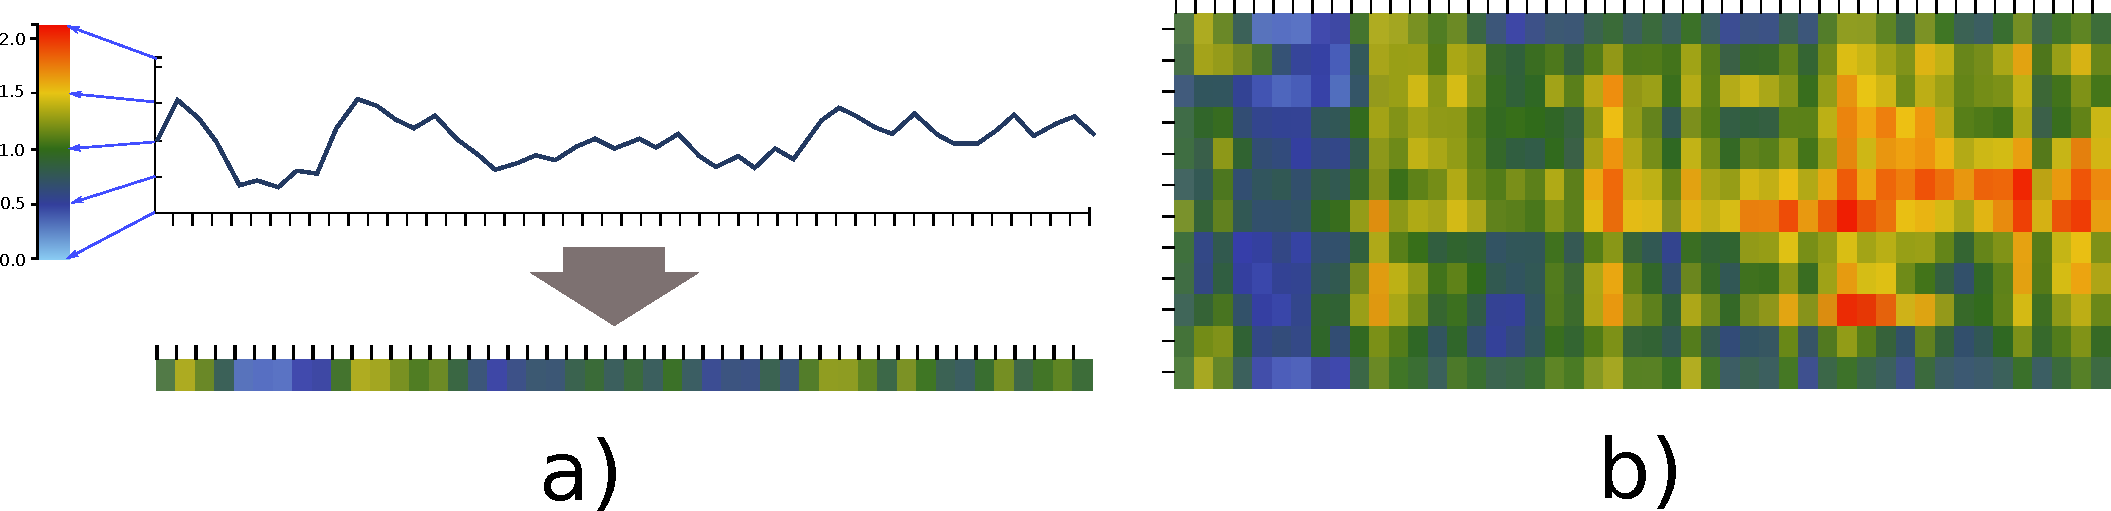
\includegraphics[width = 7.0in, height = 2.2in]{colormap}
	\caption{a) Konštrukcia jedného pásu zobrazením hodnôt grafu na farebnú škálu b) Výsledná vizualizácia, ako farebná mapa }
	\label{fig:colormap}
\end{figure}

\subsection{Detail štatistík {\small(\textit{Mnoho-čiarový diagram})}}
Napriek tomu, že zobrazením hodnôt na farbu nestrácame žiadnu informáciu, je dokázané, že človek nedokáže tak dobre porovnávať farby, ako napríklad vzdialenosti. Preto predošle spomenutá technika je síce vhodná na preskúmanie celého intervalu ako celku, avšak nie na detailné porovnávanie hodnôt v čase. Z tohto dôvodu sme sa rozhodli použiť taktiež spomínaný čiarový diagram. 

Tento typ diagramu poskytuje dostatočne veľký vizuálny priestor na to, aby sme doň mohli pridať ďalšie dáta. Rozhodli sme sa preto umožniť užívateľovi vizualizovať buď rôzne druhy štatistík súčasne pre danú predpoveď a veličinu (napr RMSE, MAE, MFE), alebo tiež rôzne veličiny (napr. tlak, teplotu, zrážky) pre túto predpoveď. V prvom prípade nám postačí jednotná škála, keďže sa hodnoty zväčša nachádzajú v podobnom rozmedzí. V druhom prípade je potrebných viacero škál, keďže napríklad chyby teploty sa pohybujú v rozmedzí 5 stupňov, tak chyby tlaku sa pohybujú v rozmedzí stoviek. Ak by sme tieto dve veličiny vizualizovali spolu, tak krivka teploty by bola sploštená natoľko, že by nebolo možné z nej odčítať hodnoty.

Vytvorenie mnoho-čiarového diagramu s jednotnou škálou je jednoduché, keďže sa na dizajne grafu nič nemení, len sa pridá ďalšia krivka. Pri viacerých rôznych škálach sa musia zobraziť aj tieto škály. Zvyčajne sa umiestňujú striedavo vľavo a vpravo, postupne za sebou smerom od stredu grafu. Problém však spočíva v tom, že pri väčšom počte nemôžme určiť, ktorá škála patrí ku ktorej krivke a s postupujúcou vzdialenosťou škály od grafu sa znižuje schopnosť užívateľa odčítavať hodnoty zo škály. V našej práci sme navrhli jednoduché spôsob, akým sme sa pokúsili vyriešiť oba problémy súčasne.

Naše riešenie spočíva v tom, že každá škála sa zobrazí ako obdĺžnik vyplnený farbou krivky, ktorá prislúcha k danej škále. Taktiež čiaročky indikujúce hodnoty v danom bode sa zobrazia pravidelne a v rovnakej vzdialenosti pre každú škálu.

Na obrázku \ref{fig:multilinegraph} môžme vidieť porovnanie bežne používaného spôsobu zobrazenia škál a nášho spôsobu. Náš spôsob jednoznačne priraďuje, pomocou farby, krivky ku škálam a jednotné, pravidelné rozmiestnenie indikátorov hodnôt nám rieši problém pri odčítavaní hodnôt, keďže nie je potrebné sa dívať na vzdialené škály.


\begin{figure}
	\centering
	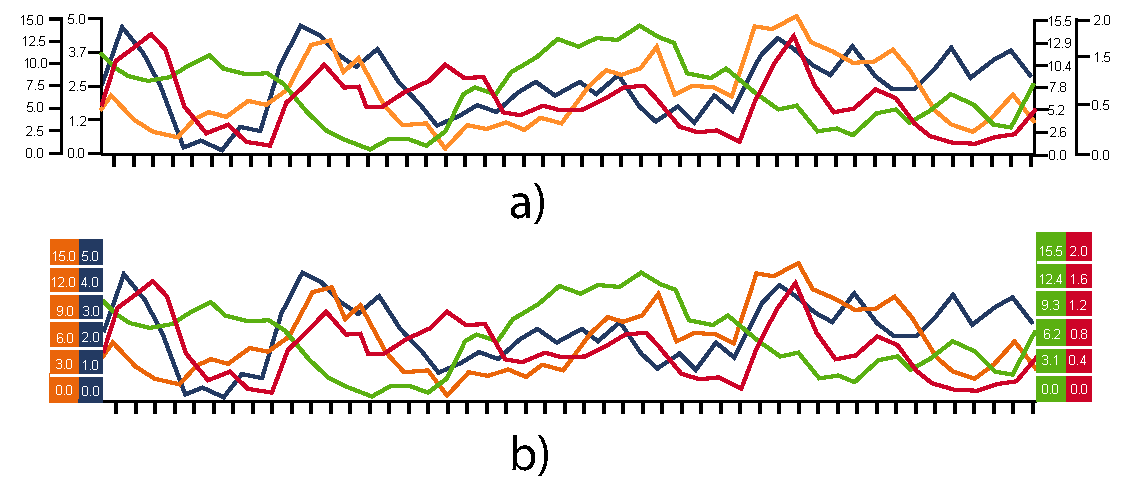
\includegraphics[width = 5in]{multilinegraph}
	\caption{a) Bežné zobrazenie viacerých škál b) Nami navrhnuté zobrazenie viacerých škál }
	\label{fig:multilinegraph} 
\end{figure}

\section{Návrh vizualizácie distribúcie chýb}
Pri verifikácii predpovede spojitej premennej sme použili štatistické metódy spomenuté v sekcii \ref{sec:errormeasurement}, ktorých výsledok sme následne vizualizovali. Pôvodné dáta však zostali skryté za použitým matematickým modelom, a tak sme stratili informáciu o distribúcii chyby. Pri verifikácii sa štandardne používajú tri metódy na priamu, či nepriamu vizualizáciu a analýzu distribúcie, ktoré sme opísali v kapitole \ref{chap:prevvis}. Týmito metódami sú bodový graf (pozri sekciu \ref{sec:scatterplot}), krabicový diagram (pozri sekciu \ref{sec:boxplot}) a histogram (pozri sekciu \ref{sec:histogram}).

My sme sa rozhodli napasovať vizualizáciu priamo na dáta verifikácie a pri jej návrhu sme vyskúšali niekoľko vizualizačných techník a zvážili ich silné a slabé stránky. 

\subsection{Graf hustoty} %Density plot

Jedným z viacerých spôsobov, ako pomerne presne určiť distribúciu chýb je pomocou \textit{grafu hustoty}. Ten sa skonštruuje jednoducho z \textit{funkcie hustoty}, ktorú získame \textit{odhadom hustoty} z dát. 

Prvý pohľad na dáta by nám vravel, že ide o dvojrozmerné dáta a teda je potrebné použiť odhad hustoty dvoch premenných. Takýto postup by samozrejme bol možný, ale doviedol by nás k chybnej vizualizácii a tak aj k mylnej predstave o dátach. Dôvodom je to, že máme záujem o analýzu distribúcie chýb pre každú hodinu predpovede zvlášť, čo znamená, že chcem zistiť distribúciu iba v jednom smere.

Pre vytvorenie grafu hustoty, v prvom rade je potrebné vybrať správny spôsob odhadu hustoty. Jedným z bežne používaným štandardným spôsobom je odhad hustoty pomocou jadra, po anglicky známy ako \textit{kernel density estimation} (KDE) [ref Rosenblatt 56, parzen 62].

Nech máme $ n $ hodnôt $ x_{i}, 1 \leq i \leq n $, z ktorých chceme určiť odhad hustoty, potom estimátor hustoty $ \hat{f}_h(x) $, ktorý aproximuje \textit{funkciu hustoty pravdepodobnosti} (PDF) $ f $, sa vypočíta takto:
\[
	\hat{f}_h(x) = \dfrac{1}{nh} \sum_{i=0}^{n}K\Big(\dfrac{x - x_{i}}{h}\Big)
\]
kde $ h $ je šírka jadra a $ K(x) $ je funkcia jadra (skrátene iba jadro), ktorá by mala spĺňať nasledovné vlastnosti:
\[  K(x) \geq 0 \]
\[  \int K(x) dx = 1 \]
tieto vlastnosti hovoria, že $ K(x) $ je na celom definičnom obore nezáporná a jej integrál je rovný 1, teda sa jedná o normalizovanú funkciu. Bolo preštudovaných mnoho jadier, ako napríklad uniformné, tri-angulárne, Epanechnikovo \cite{Turlach}, kvadratické, Gaussové, kosínusové a veľa ďalších. Najbežnejšie a zrejme aj najpraktickejšie \cite{Minnotte} je Gaussovo (normálne) jadro, ktoré sme použili aj my:
\[
	K(x) = \dfrac{1}{\sqrt{2\pi}}e^{-\frac{1}{2}x^2}
\]
Voľba jadra však nemá na výsledok až taký vplyv, ako voľba šírky jadra $ h $. My sme použili výpočet šírky jadra na základe dátovej množiny, ktorý aproximuje optimálnu šírku jadra \cite{Scott, BowmanAzzalani} \footnote{Optimálna šírka jadra je taká, ktorá minimalizuje \textit{strednú integrovanú kvadratickú chybu}.}. Všeobecne pre $ d $ dimenzionálne dáta je vzorec nasledovný:
\[
	h = \sigma \Big(\frac{4}{(d + 2)n}\Big)^{\frac{1}{d+4}}
\]
kde $ \sigma $ je smerodajná odchýlka vypočítaná z daných dát a $ n $ je veľkosť dátovej množiny. V našom prípade je $ d = 1 $, a tak sa nám vzorec zjednoduší na
\[
	h = \sigma \Big(\dfrac{4}{3n}\Big)^{\frac{1}{5}}
\] 
Aby sme zjednodušili výpočet, tak sme si konštanty vypočítali predom a zaokrúhlili na 2 desatinné miesta, čo považujeme za dostačujúce. Výsledný vzorec, ktorý sa nakoniec objavil v aplikácii je takýto:
\[
	h = 1.06 \times \sigma \times n^{-\frac{1}{5}}
\]

Takýmto spôsobom sme si pre každú hodinu predpovede určili samostatnú funkciu $ \hat{f}_{h}(x) $, ktorú môžme vizualizovať. Zvyčajne sa funkcie hustoty vizualizujú ako bežné funkcie, teda pomocou čiarového diagramu, tak ako na obrázku \ref{fig:XY}. V našom prípade by bol tento prístup nepraktický, keďže máme veľké množstvo funkcií, tak jednak by bola takáto vizualizácia nepraktická pri porovnávaní distribúcií a taktiež na to nemáme potrebný vizuálny priestor.

Opäť sme teda zvolili štandardné riešenie, ako ušetriť vzácny priestor a to tak, že hodnoty, ktoré by boli zobrazené na $ y $-ovú os zobrazíme na zvolenú farebnú škálu. Vďaka tomu by teoreticky mohol mať graf hustoty pre jeden čas predpovede šírku 1 pixel bez straty akejkoľvek informácie.

Vieme, že pre ľudí nie je také jednoduché pozorovať malé rozdiely medzi dvoma farbami. Testovaním sme zistili, že tento fakt spôsobuje problémy aj pri našej vizualizácii, kedy sa pre pozorovateľa strácajú jemné výkyvy hodnôt. Riešením by bolo nepoužiť spojité, ale diskrétne farbenie, ktoré je rozdeľuje interval hodnôt na podintervaly, ku ktorým priradí konkrétnu farbu (pozri obr. \ref{fig:XYZ}). Výhodu je, že takéto farbenie má výraznejšie farebné rozdiely. Týmto spôsobom by sme však stratili priveľa informácie a nebolo by potrebné použiť na odhad hustoty KDE, ale postačoval by aj histogram. 

Riešenie tohto problému sme našli v práci od Takafumi Saita z roku 2005 \cite{Saito}. V tomto článku autor so svojimi kolegami navrhuje nový spôsob pseudo farbenia, ktoré nazýva \textit{two-tone pseudo coloring} alebo inak po slovensky \textit{dvojtónové pseudo farbenie}. Navrhnutá metóda priraďuje každej hodnote intervalu dve výrazne rôzne farby resp. farebné časti. Toto sa uskutočňuje podobne ako pri spojitom farbení, avšak sa neinterpolujú farby, ale pomer veľkostí dvoch zafarbených častí. Na obrázku \ref{fig:twotone} možno vidieť porovnanie troch spomenutých techník farbenia.

\begin{figure}
	\centering
	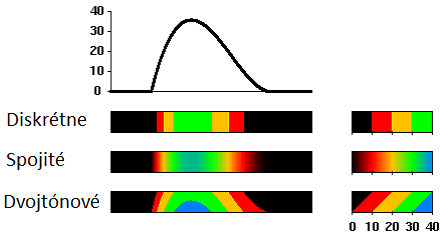
\includegraphics[width = 3.5in]{twotone}
	\caption{Porovnanie dvoch konvenčných techník farbenia so Saitovým dvojtónovým farbením. Obrázok pochádza z pôvodného článku \cite{Saito}. }
	\label{fig:twotone} 
\end{figure}

%TODO Ďalší problém - nevidno hranice!. 

Na obrázku \ref{fig:XYZ} vodno porovnanie vizualizácií s použitím spojitého a dvojtónového farbenia.

\subsection{Pruhový kvantilový diagram} 
Z časti \ref{subsec:scatterplot} sme už dobre oboznámený s pojmom kvantil. Klasický kvantilový diagram [ref] zobrazuje kvantil hodnôt pre jednu dimenziu. Ak si vezmeme naše dáta, kde pre každý čas je niekoľko chýb predpovedí, tak kvantilový diagram skonštruujeme tak, že pre každý čas vypočítame kvantil, ktorý zobrazíme ako bod alebo ako súčasť lomenej čiary v grafe.
Prirodzeným rozšírením je zobrazovať nielen jeden kvantil, ale mnoho kvantilov súčasne. Zvyčajne sú to tieto kvantily $ Q_{0.02}, Q_{0.98}, Q_{0.25}, Q_{0.75}, Q_{0.5} $. V našej práci sme využili toto rozšírenie na lepšie zobrazenie distribúcie a navrhli sme takzvaný \textit{pruhový kvantilový diagram}.

Jeden \textit{pruh} v grafe definujeme pomocou dvojíc hodnôt v čase - spodným a jeho protiľahlým kvantilom. Spodným kvantilom je kvantil $ Q_{\alpha} $ a k nemu protiľahlý je kvantil $ Q_{1 - \alpha} $, kde $ 0 \leq \alpha \leq \frac{1}{2} $. Vidíme teda, že pruh ohraničuje hodnoty v okolí stredu usporiadanej množiny dát. Špeciálnym prípadom pruhu je pre $ \alpha = \frac{1}{2} $, vtedy spodný aj horný kvantil je $ Q_{0.5} $, čo je vlastne medián.

Pri návrhu vizualizácie sme sa snažili, aby mohol mať diagram variabilný počet pruhov a taktiež, aby rozostup medzi pruhmi bol pravidelný. Pri riešení tohto problému, sme sa inšpirovali krabicovým diagramom, kde sa hodnoty delia mediánom na dve časti, ktoré sa ďalej taktiež delia ich mediánom. Ide teda o rekurzívne delenie usporiadanej množiny na polovicu do hĺbky 2. Túto myšlienku sme rozšírili na ľubovoľnú hĺbku delenia $ d $. Potom $ i $-ty pruh $ \mathcal{P}_{d}(i) $ pre hĺbku $ d $ definujeme takto:
\[
	p_{d}(i) = (Q_{\alpha},Q_{1 - \alpha}) , \alpha = i \times (0.5)^d 	
\]
\[
	\mathcal{P}_{d}(i) = \{ (t,p_{d}(i)) : t \in I \}
\]
a množina všetkých pruhov grafu pre hĺbku delenia $ d $ je definovaná takto:
\[
	\{ \mathcal{P}_{d}(i) : 0 \leq i \leq 2^{d-1} , i \in \mathbb{N} \}
\]
Aby sme sa vyhli rekruzii, vypočítali sme si krok medzi susednými kvantilmi pri hĺbke $ d $, ktorý je $ (0.5)^d $, a jednotlivé pruhy sme generovali s týmto krokom. Pri rekruzívnom delení sa vygeneruje $ 2^d $ kvantilov a z nich je možné vyrobiť $ 2^{d - 1} $ pruhov, preto sme index $ i $ obmedzili na $ i \leq 2^{d-1} $. Z tohto vidíme, že počet pruhov grafe s rastúcou hĺbkou rastie exponenciálne, preto odporúčame, aby $ d $ bolo maximálne 4, kedy sa nám množina rozdelí na 16 častí 15 hexadecilmi a tak vznikne 8 pruhov.

% TODO obrázok 
Na obrázku \ref{fig:pruh} vidíme, že takto definovaný pruh sa potom vizualizuje, ako plocha medzi krivkami, ktoré tvoria dvojice hodnôt patriace danému pruhu, s výnimkou špeciálneho prípadu $ Q_{0.5} $, ktorý vizualizujeme ako krivku.



%TODO toto musím ešte celé premyslieť!


\subsection{Funkčný krabicový diagram}
Pre pochopenie dát je dôležité, aby sme sa vedeli pozrieť na hodnoty v ich kontexte. Všetky predošlé techniky uvažovali o chybe ako o samostatnej hodnote pre určitý predpovedný čas, avšak chyby sa nenachádzajú len v kontexte predpovedného času, ale aj v kontexte konkrétnej predpovede. Preto môžme uvažovať o predpovediach ako o funkciách $ x_{i}(t) $, kde $ i \in \{1..n\}$ je poradie predpovede a $ t \in I $ je čas predpovede, kde $ I $ je časový interval predpovede z $ \mathbb{R} $ (v našom prípade sa jednalo o dvojdňovú, teda 48 hodinovú predpoveď).

Takýmto spôsobom sme sa dostali do novej situácie, kedy nechceme vizualizovať distribúciu jednotlivých chýb, ale celých predpovedí, ktoré chápeme ako funkcie. Na riešenie tohto problému existuje niekoľko spôsobov, z ktorých sme si zvolili \textit{funkčný krabicový diagram} \cite{FunctionalBoxplot}, keďže myšlienkovo vychádza z klasického krabicového diagramu, ktorý je jednak na túto situáciu vhodný ale je tiež medzi užívateľmi dobre známy a zaužívaný.

Ako sme spomenuli v časti \ref{subsec:boxplot}, klasický krabicový diagram potrebuje na svoju konštrukciu 5 hodnôt: 3 kvartily a 2 extrémy. Aby sme tieto hodnoty našli pre funkcie, musíme ich vedieť porovnať a povedať, ktorá je \textquotedblleft väčšia\textquotedblright alebo \textquotedblleft menšia\textquotedblright. Autori funkčného krabicového diagramu riešia problém s využitím takzvanej pásmovej hĺbky (\textit{band depth}) \cite{BandDepth}. Grafom $ G $ funkcie $ x $ je množina bodov $ G = \{ (t,x(t)) : t \in I \} $. Pásmo $ \mathcal{B} $ (\textit{band}) v $ \mathbb{R}^{2}  $ ohraničené krivkami $ x_{i_{1}}, x_{i_{2}}, .. , x_{i_{k}} $, kde $ k \geq 2 $ je definované takto:
\[
	\mathcal{B}(x_{i_{1}}, x_{i_{2}}, .. , x_{i_{k}}) = \{ (t,y) : t \in I, \min_{r=1..k}x_{i_{r}}(t) \leq y \leq \min_{r=1..k}x_{i_{r}}(t) \}
\]
Pásmo $ \mathcal{B} $ je teda množina všetkých bodov existujúcich medzi extrémami všetkých kriviek, ktoré doň vstupujú ako parameter. 
Pomocou týchto dvoch funkcií môžme definovať pomocnú funkciu $ BD_{n}^{(j)}(x) $ pre krivku $ x $, ktorá vyzerá takto:
\[
	BD^{(j)}_{n}(x) = {n \choose j}^{-1} \sum_{1 \leq i_{1} < i_{2} < ... < i_{j} \leq n} \mathcal{I}\{ G(x) \subset \mathcal{B}(x_{i_{1}}, ... ,x_{i_{j}}) \}, j \geq 2
\]
kde $ j $ je počet kriviek definujúce pásmo $ \mathcal{B} $, $ n $ je celkový počet kriviek a $ \mathcal{I} $ je takáto funkcia:
\[
	\mathcal{I}(x) = \left\{
	\begin{array}{ll}
	1 & \mbox{ak platí x}  \\
	0 & \mbox{ak neplatí x} 
	\end{array}
	\right.
\]
Pomocná funkcia $ BD $ pre krivku $ x $ definuje pomer všetkých pásem zložených z $ j $ kriviek, v ktorých sa graf $ G(x) $ nachádza, ku všetkým možným $ j $-ticiam kriviek vybraným z $ n $. 
Samotná funkcia pásmovej hĺbky $ \mathcal{BD} $ pre krivku $ x $ je definovaná takto:
\[
	\mathcal{BD}_{n, J}(x) = \sum_{j = 2}^{J} BD^{(j)}_{n}(x), J \geq 2
\]
Hĺbka pásma $ \mathcal{BD} $ je teda suma všetkých $ BD $ pre počet kriviek 2 až $ J $.

Autor článku definujúci pojem pásmová hĺbka navrhol taktiež flexibilnejšiu verziu s použitím pomocnej funkcie $ MBD $ (\textit{modified band depth}) \cite{BandDepth}. V pravom rade je potrebné zadefinovať si funkciu $ A $, ktorá určí všetky časové body, kedy sa krivka $ x $ nachádza v pásme $ B $.
\[
	A(x, B) = \{ t \in I : (t, x(t)) \in G(x) \wedge (t, x(t)) \in B \}
\]
V spomínanom článku autori využívajú alternatívnu definíciu funkcie $ A $, do ktorej vstupuje $ j + 1 $ kriviek. Jej význam zostáva rovnaký ako pri našej definícii, avšak náš prístup považujeme za jednoduchší a zrozumiteľnejší. S využitím \textit{Lebesguevoej miery} $ \lambda $ autori ďalej definujú funkciu $ \lambda_{r} $, ktorá nám dáva "pomer času, ktorý krivka strávi v pásme":
\[
	\lambda_{r}(A) = \dfrac{\lambda(A)}{\lambda(I)} 
\]
Nová pomocná funkcia $ MBD $ je definovaná nasledovne:
\[
	MBD^{(j)}_{n}(x) = {n \choose j}^{-1} \sum_{1 \leq i_{1} < i_{2} < ... < i_{j} \leq n} \lambda_{r}\{ A(x, \mathcal{B}(x_{i_{1}}, ... ,x_{i_{j}})) \}, j \geq 2
\]
Ak platí, že $ G(x) \subset \mathcal{B}(x_{i_{1}}, ... ,x_{i_{j}}) $, tak funkcia $ MBD $ sa degeneruje na $ BD $ \cite{FunctionalBoxplot}.

V našej aplikácii sme sa rozhodli, že budeme pásmo definovať pomocou iba dvoch kriviek, čo nám vzorec výrazne zjednodušilo. Taktiež to implikovalo fakt, že pri výpočte $ MBD $ nie je potrebné $ {n \choose j}^{-1} $, keďže berieme pásma zložené vždy z rovnakého počtu kriviek. Pre naše účely sme si taktiež zjednodušili funkciu $ \lambda_{r} $ na $ \lambda $, keďže nepotrebujeme vlastnosť tejto funkcie, ktorá dosahovala to, že $ MBD $ pre špeciálny prípad degeneruje na $ BD $. Po týchto úpravách výsledný vzorec pre naše $ \mathcal{BD}' $ vyzerá nasledovne:
\[
	\mathcal{BD}'_{n}(x) = \sum_{1 \leq i_{1} < i_{2} \leq n} \lambda\{ A(x, \mathcal{B}(x_{i_{1}},x_{i_{2}})) \}
\]
Teraz, keď sme úspešne definovali mieru, podľa ktorej môžme usporiadať funkcie resp. ich krivky, je veľmi ľahké skonštruovať funkčný krabicový diagram.

\paragraph{}
Nech sú naše funkcie predpovedí $ x_{1},.., x_{n} $ usporiadané zostupne podľa $ \mathcal{BD}' $. Potom krivka pre funkciu $ x_{1} $ má najvyššiu pásmovú hĺbku a predstavuje strednú hodnotu pre množinu funkcií, teda niečo podobné ako medián hodnôt pri krabicovom diagrame. Pri konštrukcii funkcionálneho diagramu nám taktiež pomôže koncept centrálneho regiónu \cite{Liu}. Centrálny región $ C $ pre 50\% kriviek je pásmo vytvorené z 50\% najhlbších kriviek, teda:
\[
	C_{0.5} = B(x_{1}, x_{2}, .., x_{\lceil n / 2 \rceil} )
\] 
Vidíme, že Centrálny región $ C_{0.5} $ zaobaľuje 50\% najhlbších kriviek, a teda sa jedná o akúsi analógiu pre medzikvartálový rozsah (IQR) v klasickom krabicovom diagrame (pozri sekciu \ref{subsec:boxplot}), ktorý ohraničoval 50\% centrálnych dát. Zobrazením hraničných bodov tohto regiónu získame obálku myšlienkovo totožnú boxu v krabicovom diagrame (pozri obrázok \ref{fig:functionalboxplot}b) ). Táto myšlienka sa dá použiť ďalej a môžme, tak ako na obrázku \ref{fig:functionalboxplot}c) , zobraziť taktiež 25\%-ný a 75\%-ný centrálny región $ C_{0.25} $, $ C_{0.75} $, avšak kvôli nižšej čitateľnosti grafu sme túto alternatívu nepoužili.

V prípade, že nepotrebujeme identifikovať \textit{outlier}-ov, tak extremálne hodnoty je už veľmi jednoduché získať, pretože ich tvorí pásmo zložené zo všetkých kriviek $ B(x_{1}, .., x_{n}) $. V opačnom prípade musíme najprv identifikovať \textit{outlier}-ov, ktorých potom vylúčime z výpočtov. Opäť sa využíva myšlienka z klasického krabicového diagramu, kedy sa \textit{outlier} určil pomocou hodnoty $ c \times IQR $, kde $ c $ bolo zvyčajne 1.5. Hranice sa teda získajú naškálovaním centrálneho regiónu so škálovacím faktorom 1.5 a všetky krivky, ktoré sa v tomto regióne nenachádzajú, budú považované za \textit{outlier}-ov. Test na \textit{outlier}-a vyzerá teda takto:
\[	y_{i}(t) = 1.5 \times x_{i}(t) \]
\[	isOutlier(x) = [ G(x) \nsubseteq B(y_{1},..,y_{\lceil n / 2 \rceil}) ] \]
Na obrázku \ref{fig:functionalboxplot}b) môžme vidieť červené prerušované čiary, ktorými sú \textit{outlier}-i znázornené.

V našej práci sme do diagramu pridali ešte jednu krivku pre ľubovoľnú štatistiku vypočítanú z chýb ako napríklad MFE, MAE alebo RMSE (pozri sekciu \ref{sec:errormeasurement}). Takto môžme spraviť porovnanie distribúcie chýb s vypočítanou štatistikou.
%TODO to je troška klamstvo ne?


\begin{figure}
	\centering
	\hspace*{-0.9in}
	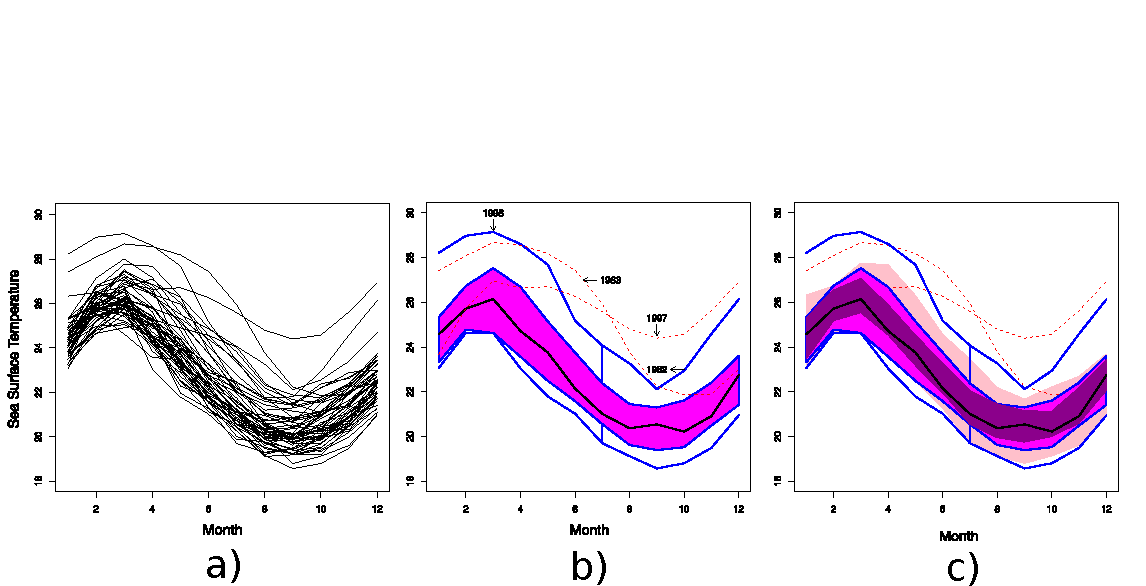
\includegraphics[width = 7.5in]{functionalboxplot}
	\caption{Obrázky z článku \textit{Functional Boxplots}  \cite{FunctionalBoxplot}  a) Funkcie meraní teploty hladiny mora b) Funkčný krabicový diagram c) Rozšírený Funkčný krabicový diagram o centrálne regióny $ C_{0.25} $ a $ C_{0.75} $ }
	\label{fig:functionalboxplot}
\end{figure}

%TODO obrazok pasmo

\subsection{Mapa distribúcií} 
Návrh tejto metódy spočíva v tom, že vizualizácia prehľadu štatistík pomocou farebnej mapy ponecháva ešte dostatok nevyužitého vizuálneho priestoru. Obsah obdĺžnikov, ktoré tvoria túto mapu, sa dá zaplniť ďalším vizuálnym elementom, ktorým je možné dodať informáciu o distribúcii.

Malý priestor však neponúka príliš veľa možností na veľký detail. Rozhodli sme sa preto poskytnúť užívateľovi informáciu o distribúcii pomocou jedinej hodnoty, konkrétne štandardnej odchýlky $ \sigma $. 
\[
	\sigma = \sqrt{\frac{1}{n} \sum_{i=1}^{n}(x_{i} - \bar{x}_{i})^2  }
\]
Jednotlivé hodnoti sa zobrazia vo vizualizácii ako kruhy rôznej veľkosti v závislosti od $ \sigma $. Ľudský percepčný systém vníma veľkosť kruhu v zmysle plochy, preto nezobrazujeme hodnoty $ \sigma $ priamo na veľkosť polomeru $ r $, ale na obsah kruhu. Vzťah, ktorým vypočítame polomer je odvodený od vzorca pre obsah kruhu a vyzerá nasledovne:
\[
	r = \sqrt{\frac{S}{\pi}}
\]
\[
	S = k\sigma
\]
kde $ k $ je koeficient škálovania. Nemusíme sa báť záporných hodnôt pod odmocninou, keďže $ \sigma $ nemôže nadobúdať záporné hodnoty a $ k > 0 $.

Takýmto spôsobom dodáme užívateľovi rýchly prehľad o tom, ako môže štatistikám z chýb dôverovať, aké sú trendy alebo vzory v disperzii a podobne. Tento typ vizualizácie sa dá kombinovať s farebnou mapou, ale môže existovať aj samostatne podľa preferencií užívateľa. Na obrázku \ref{fig:XYZ} je znázornený príklad výslednej vizualizácie.


\subsection{Porovnanie metód}

Tu bude pekný obrázok a obkeci. \\
Graf hustoty je presnejsi, ale menej citatelny. \\
Pruhovy kvantilovy diagram nahradzuje krabicovy diagram. \\
Funkcionalny krabicovy riesi distribuciu funkcii. \\

Pre pruhovy nezabudnut, ze \cite{Bade} spravil nieco podobne.

alebo to sem vobec nedam! 

\section{Návrh farebnej palety}
Farba je pravdepodobne najviac podceňovaný a nesprávne používaný vizuálny parameter vo vizualizácii dát. V tejto časti opisujeme návrh farebnej palety pre vyššie spomenuté vizualizačné techniky.

\subsection{Farebná mapa}
Návrhu farebnej palety pre farebnú mapu sme venovali zvýšenú pozornosť, keďže farba hrá pri tomto type vizualizácie najpodstatnejšiu úlohu.

V prvom momente sme siahli po veľmi prvoplánovom riešení a použili sme takzvanú \textit{dúhovú farebnú škálu}, ktorú možno vidieť v sekcii \ref{sec:colormap} na obrázku \ref{fig:colormap}. Výskum ukázal a mnohý vedci sa na tom zhodujú, že tento typ farebnej palety je len zriedkakedy najlepšia voľba pri vizualizácii. Dúhové farebné palety majú niekoľko slabých stránok, ktoré zhŕňa David Borland a Russell M. Taylor II vo svojom článku \cite{RainbowHarmful}.

Prvou slabinou je, že farby v dúhovej palete, narozdiel od monochromatickej, nemajú jasný kľúč podľa ktorého by sme ich perceptuálne zoradili. Preto základné vzťahy \textit{menší ako}, \textit{väčší ako} nie sú ihneď evidentné. Ľudský vizuálny systém vníma vysoké priestorové frekvencie prostredníctvom zmien v jase. Z tohto vyplýva ďalší problém, pretože dúhová paleta zakrýva detail tým, že zmeny medzi hodnotami zobrazuje ako zmenu vo farebnom odtieni a nie ako zmenu v jase. Poslednou, v článku spomenutou, slabinou je, že farby v dúhovej palete sa spájajú do pásem, čím pridáva do obrazu artefakty, ktoré sa nevyskytovali v pôvodných dátach. 

Týchto niekoľko závažných dôvodov nás presvedčilo zvoliť inú farebnú paletu. Konkrétne sme sa rozhodli použiť divergentnú farebnú paletu zloženú z troch farieb: červená, biela a modrá. Červená znázorňuje kladné maximum, biela hodnoty blízko nuly a modrá záporné maximum. Výber týchto troch farieb bol jednoduchý, pretože červená farba zvyčajne indikuje kladné hodnoty a naopak modrá záporné. Smerom k nule sa potom už iba zvyšuje jasová zložka farby, až kým nedosiahneme bielu. Konkrétne farby sme vybrali z internetovej galérie farebných paliet, ktorú zverejnil \textit{NCAR} (\url{http://www.ncl.ucar.edu/Document/Graphics/color_table_gallery.shtml}).

Tento typ palety už lepšie zodpovedal našim požiadavkám. Testovaním sme však zistili, že nie je jednoduché ihneď rozoznať záporné oproti kladným hodnotám, ktoré sú blízko nuly a naopak. Vyriešili sme to nahradením bielej farby dvoma rôznymi farbami. Jednak svetlo modrou pre hodnoty blížiace sa k nule z dola a svetlo červenou pre hodnoty blížiace sa k nule zhora. Vďaka tomu na farebnej škále a rovnako aj vo vizualizácii vznikol ostrý predel medzi kladnými a zápornými hodnotami. Na obrázku \ref{fig:colorpalettes} môžme vidieť porovnanie týchto troch farebných paliet.


\begin{figure}
	\centering
	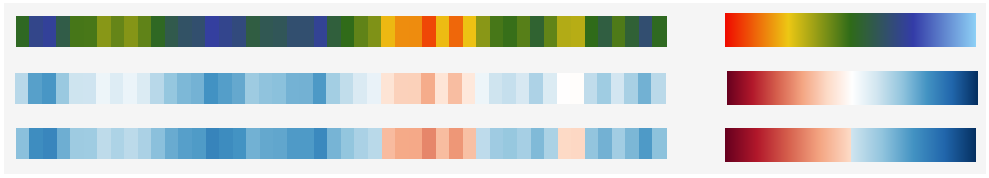
\includegraphics[width = 5in]{colorpalettes}
	\caption{Vývoj farebnej palety pre farebnú mapu}
	\label{fig:colorpalettes}
\end{figure}

- ekvalizacia histogramom / boxplotom ??? \\

\subsection{Ďalšie diagramy}
Podobné uvažovanie ako pre farebnú mapu sme aplikovali aj pre ďalšie diagramy. Vzhľadom na to, že vo zvyšných diagramoch nehrajú farby takú výraznú úlohu, v tejto kapitole stručne zhrnieme dôvody, ktoré nás viedli k výberu farieb pre jednotlivé diagramy.

\subsubsection{Mnoho-čiarový diagram} 
Tento typ diagramu sme použili v dvoch prípadoch. Pre hodnoty štatistík na jeden mesiac a pre priebeh chýb počas roka.

V prvom prípade na farbe takmer vôbec nezáleží, jedine pri použití rôznych škál, kedy sme volili tmavšie odtiene, aby bolo vidieť biele indikátory hodnôt zobrazené na škálach.

V druhom prípade sme sa snažili zvýrazniť kĺzavý priemer červenou farbou, zatiaľ čo surové dáta sme nechali pomocou tmavo šedej ustúpiť do pozadia.

\subsubsection{Graf hustoty} 
Tento diagram zobrazuje výlučne kladné hodnoty, preto sme zvolili jednoduchú monochromatickú škálu. V tomto prípade nám poslúžil internetový nástroj \textit{Color Brewer} (\url{http://colorbrewer2.org/}), kde sme zvolili škálu v modrých odtieňoch.

\subsubsection{Pruhový diagram} 
Taktiež v tomto prípade sme zvolili monochromatickú škálu. Farby sa smerom k stredu diagramu postupne stmavujú. Pruh pre medián sme však zvýraznili žltou, ktorá vystúpila na tmavou pozadí do popredia.

\subsubsection{Funkčný krabicový diagram} 
Pri návrhu farebnej palety pre tento diagram sme vychádzali z farieb dizajnu systému, teda z modrej a bielej. Centrálne pásmo $ C_{0.5} $ má tmavomodrú farbu s bielim zobrazeným priemerom a neviem akým mediánom. %TODO neviem akym prepisaz
Otlieri sme zámerne zvýraznili červenou farbou.

\section{Návrh rozloženia prvkov vizualizácie}
Výsledná obrazovka systému sa nebude skladať iba z jedného typu vizualizácie, ale z viacerých grafov a iných častí, ktoré spolu užívateľovi vytvoria dostatočne dobrú predstavu o dátach. Tieto časti budeme nazývať prvky alebo komponenty vizualizácie. Jednotlivým prvkom sme dali nasledovné pomenovania: 

\begin{itemize}
	\item\textit{Meta informácie} je tabuľka obsahujúca informácie o stanici (Názov, geografická poloha, nadmorská výška), názov modelu, interval verifikácie, spôsob interpolácie a podobne.  
		
	\item\textit{Prehľad} je komponent vizualizácie, ktorý by mal poskytovať celistvý pohľad na všetky mesačné štatistiky. Jeho úlohou nie je detailné zobrazenie chýb, ale odhalenie vzorov, trendov a výkyvov vo fungovaní modelu počas skúmaného intervalu.
	
	\item\textit{Zjednodušený prehľad} je vo svojej podstate rovnaký ako \textit{Prehľad}. Rozdielom je však menšia plocha, ktorú zaberá, zjednodušená farebná škála a chýbajúce popisky.
	
	\item\textit{Celkový priebeh} zobrazuje priebeh chýb počas celého intervalu. Nie však z pohľadu 48 predpovedných hodín (ako \textit{Prehľad}), ale z pohľadu jednotlivých dní.
	
	\item\textit{Detail štatistík} je prvok slúžiaci na detailnejšie skúmanie štatistík počas jedného mesiaca. V grafe sa nachádzajú všetky dostupné štatistiky pre daný mesiac.
	
	\item\textit{Detail chýb} pre daný mesiac, nám dáva pohľad na chyby predpovede, z ktorých sa počítali štatistiky.
	
	\item\textit{Distribúcia chýb} sa taktiež zobrazuje pre konkrétny mesiac a týmto komponentom je graf, v ktorom je zobrazená distribúcia chýb v danom mesiaci.
\end{itemize}

 Pre lepšiu orientáciu v kapitole sme pre jednotlivé prvky priradili aj obrázkové ikony. Jednotlivé priradenia sú vyobrazené na obrázku \ref{fig:designicons}. 
 
 Pri návrhu rozloženie prvkov vizualizácie na obrazovke sme sa rozhodovali medzi dvoma smermi uvažovania, ktoré opíšeme v tejto sekcii. 

\begin{figure}
	\centering
	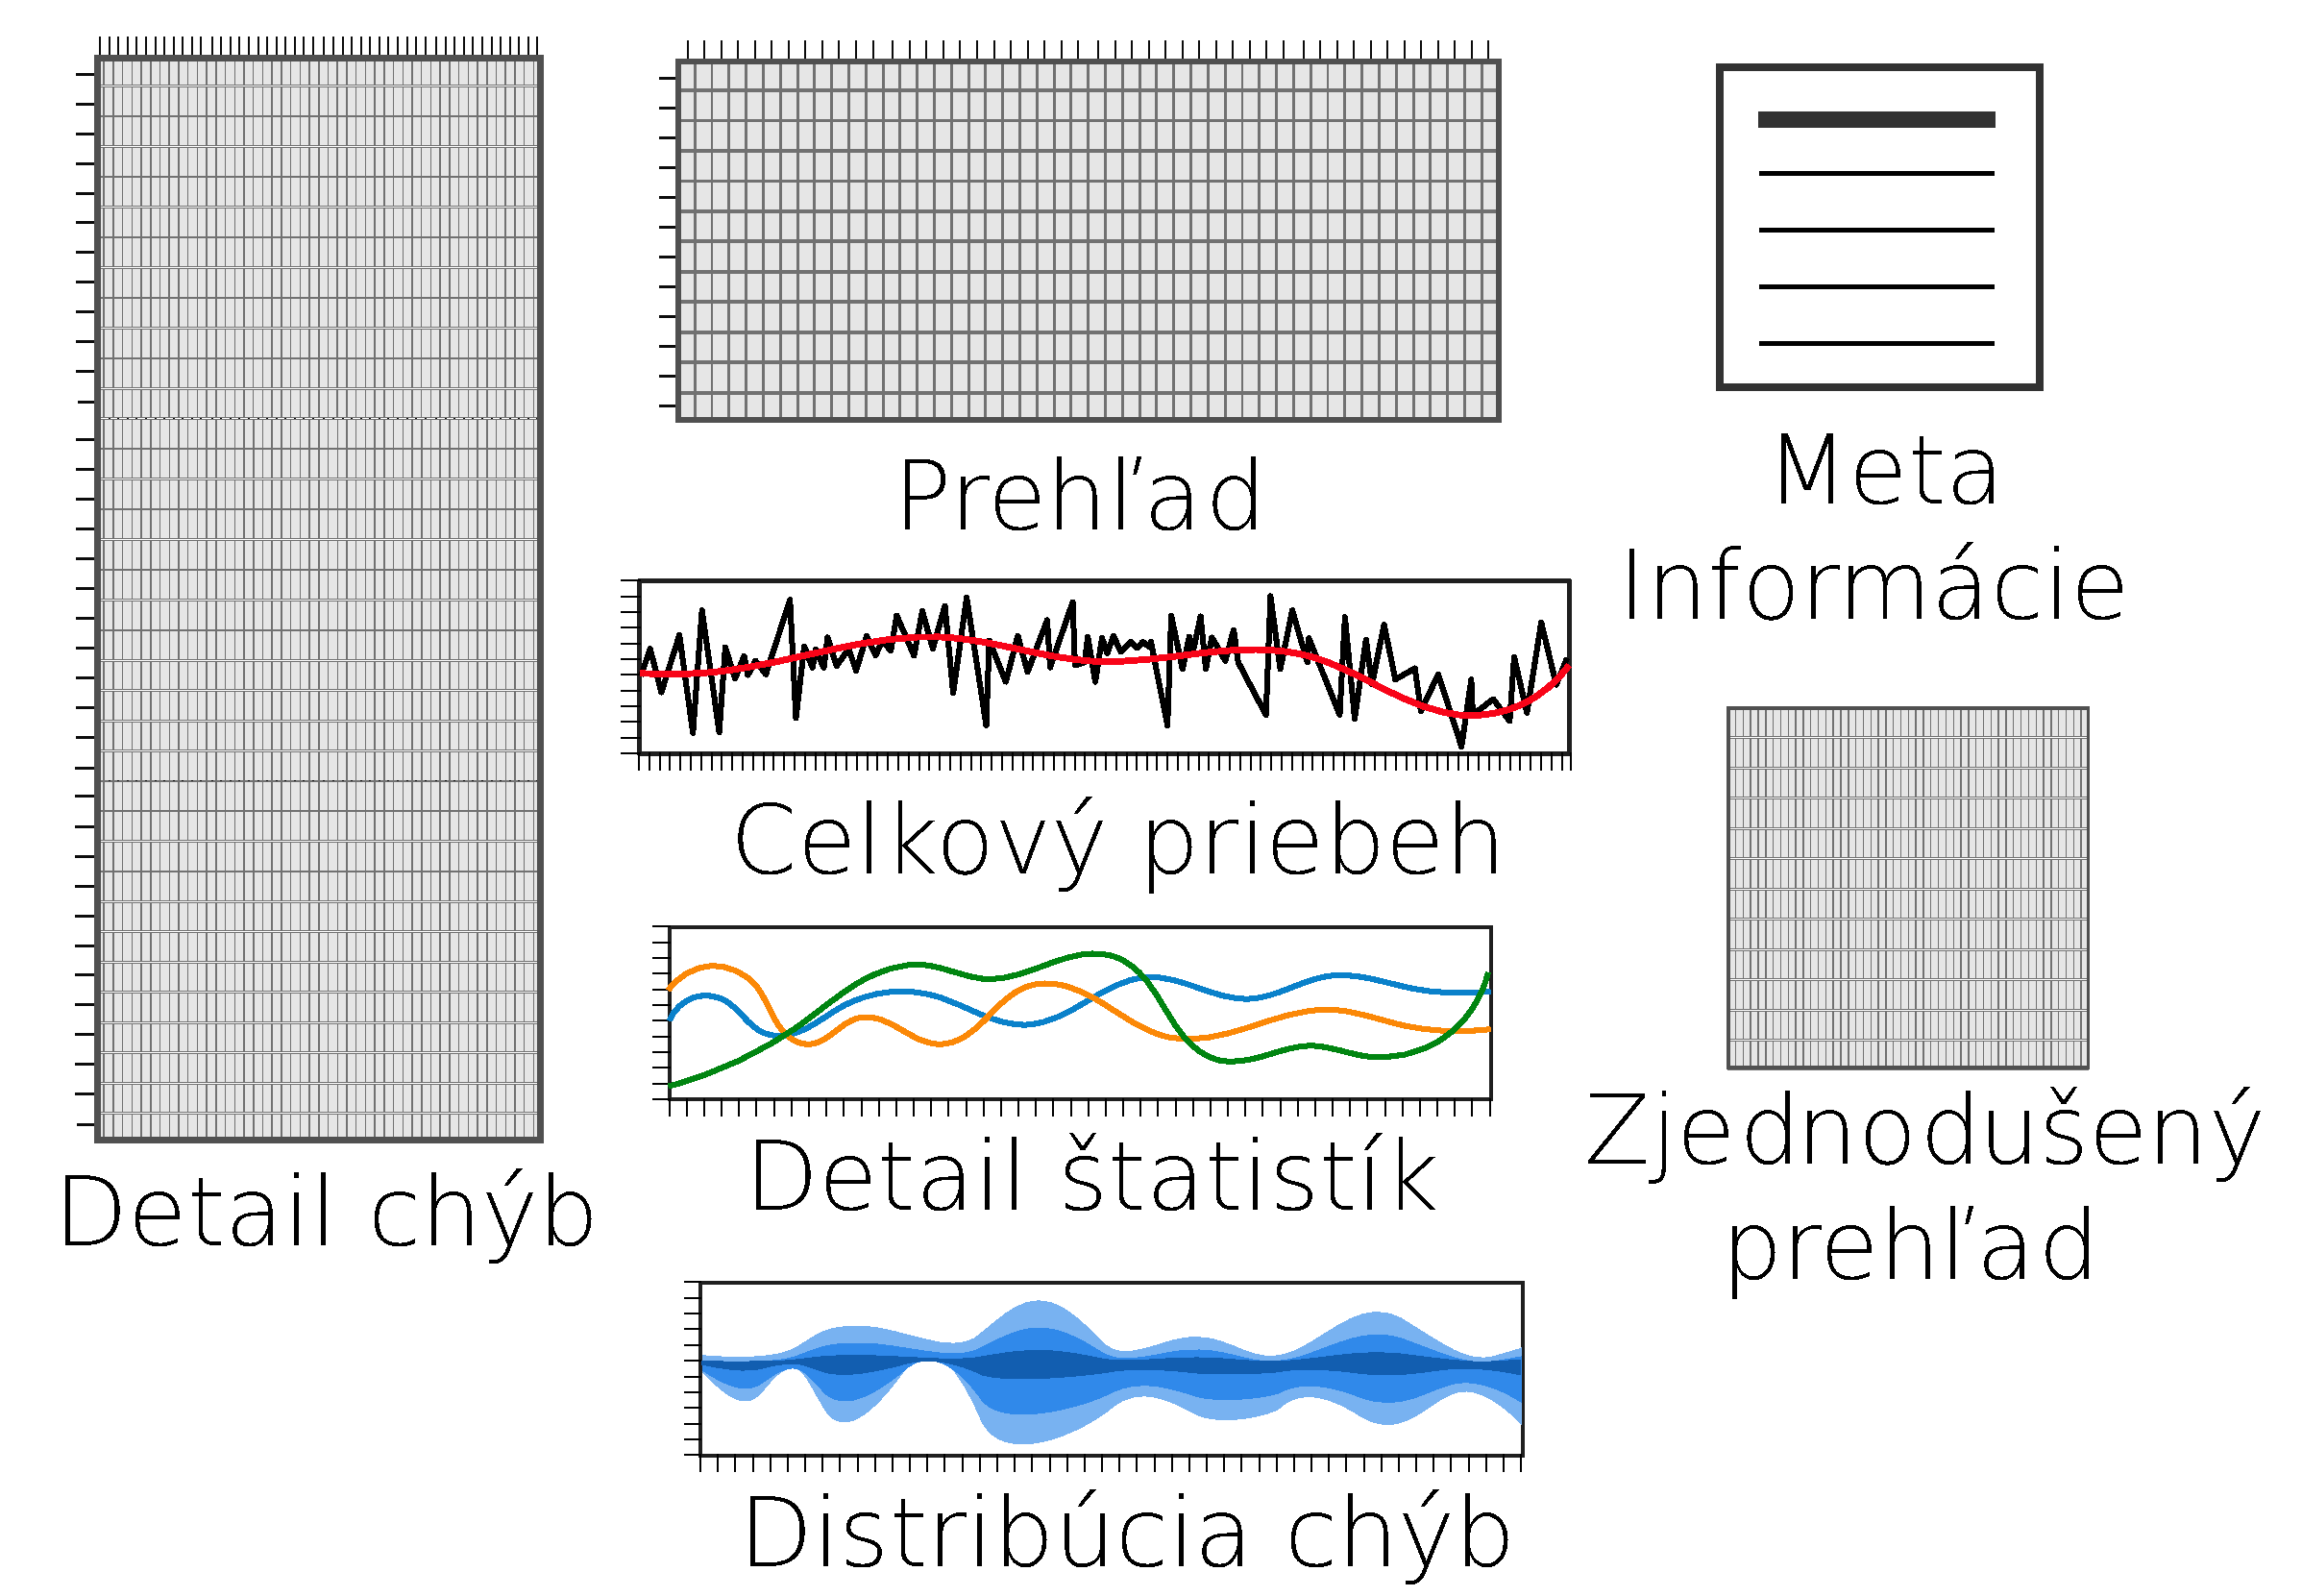
\includegraphics[width = 4.5in]{designicons}
	\caption{Ikony pre jednotlivé prvky vizualizácie}
	\label{fig:designicons}
\end{figure}


\subsection{Viacúrovňový návrh rozloženia prvkov}
Jeden zo spôsobov uvažovania, ako rozložiť prvky vizualizácie, bolo zobraziť ich v jednotlivých úrovniach detailu: 
\begin{easylist}
	# \textit{Úroveň rokov}
	# \textit{Úroveň mesiacov}
	# \textit{Úroveň štatistík}
	# \textit{Úroveň chýb} 
\end{easylist}
Každá úroveň sa skladá z jedného alebo viacerých prvkov rovnakého typu. Napríklad \textit{Úroveň rokov} obsahuje iba prvky \textit{Zjednodušený prehľad}, ktorými sa zobrazujú celé roky. Obmedzením, ktoré kladieme na tento návrh, je zobrazenie maximálne dvoch úrovní súčasne. Touto požiadavkou dosiahneme jednak to, že prvky nebudú zbytočne presahovať mimo obrazovku a taktiež sa zachová do istej miery \textit{detail a kontext}. 

Medzi jednotlivými úrovňami je možný pohyb pomocou klikaním myši na jednotlivé prvky. Napríklad úrovni rokov kliknutím na jeden rok (prvok \textit{Zjednodušený prehľad}) sa nám zobrazí ďalšia úroveň ako prvok \textit{Prehľad}. Ďalším kliknutím na jeden mesiac v danom prvku sa pre daný mesiac zobrazí úroveň štatistík, ako prvok \textit{Detail štatistík}. Ďalej po kliknutí na jednu zo štatistík sa zobrazí prvok \textit{Distribúcia chýb}, v ktorom máme detailne zobrazené chyby, z ktorých sa nám daná štatistika počítala.

Na obrázku \ref{fig:multilevellayout} máme pomocou ikon z obrázka \ref{fig:designicons} schematicky popísané jednotivé úrovne a pohyb medzi nimi. Môžme si všimnúť, že v schéme nie je vidno prvok \textit{Detail chýb}. Dôvodom je, že sa nám kvôli jeho veľkosti nepodarilo nájsť umiestnenie tohto prvku jednak medzi úrovňami a rovnako aj v rámci úrovne.

\begin{figure}
	\centering
	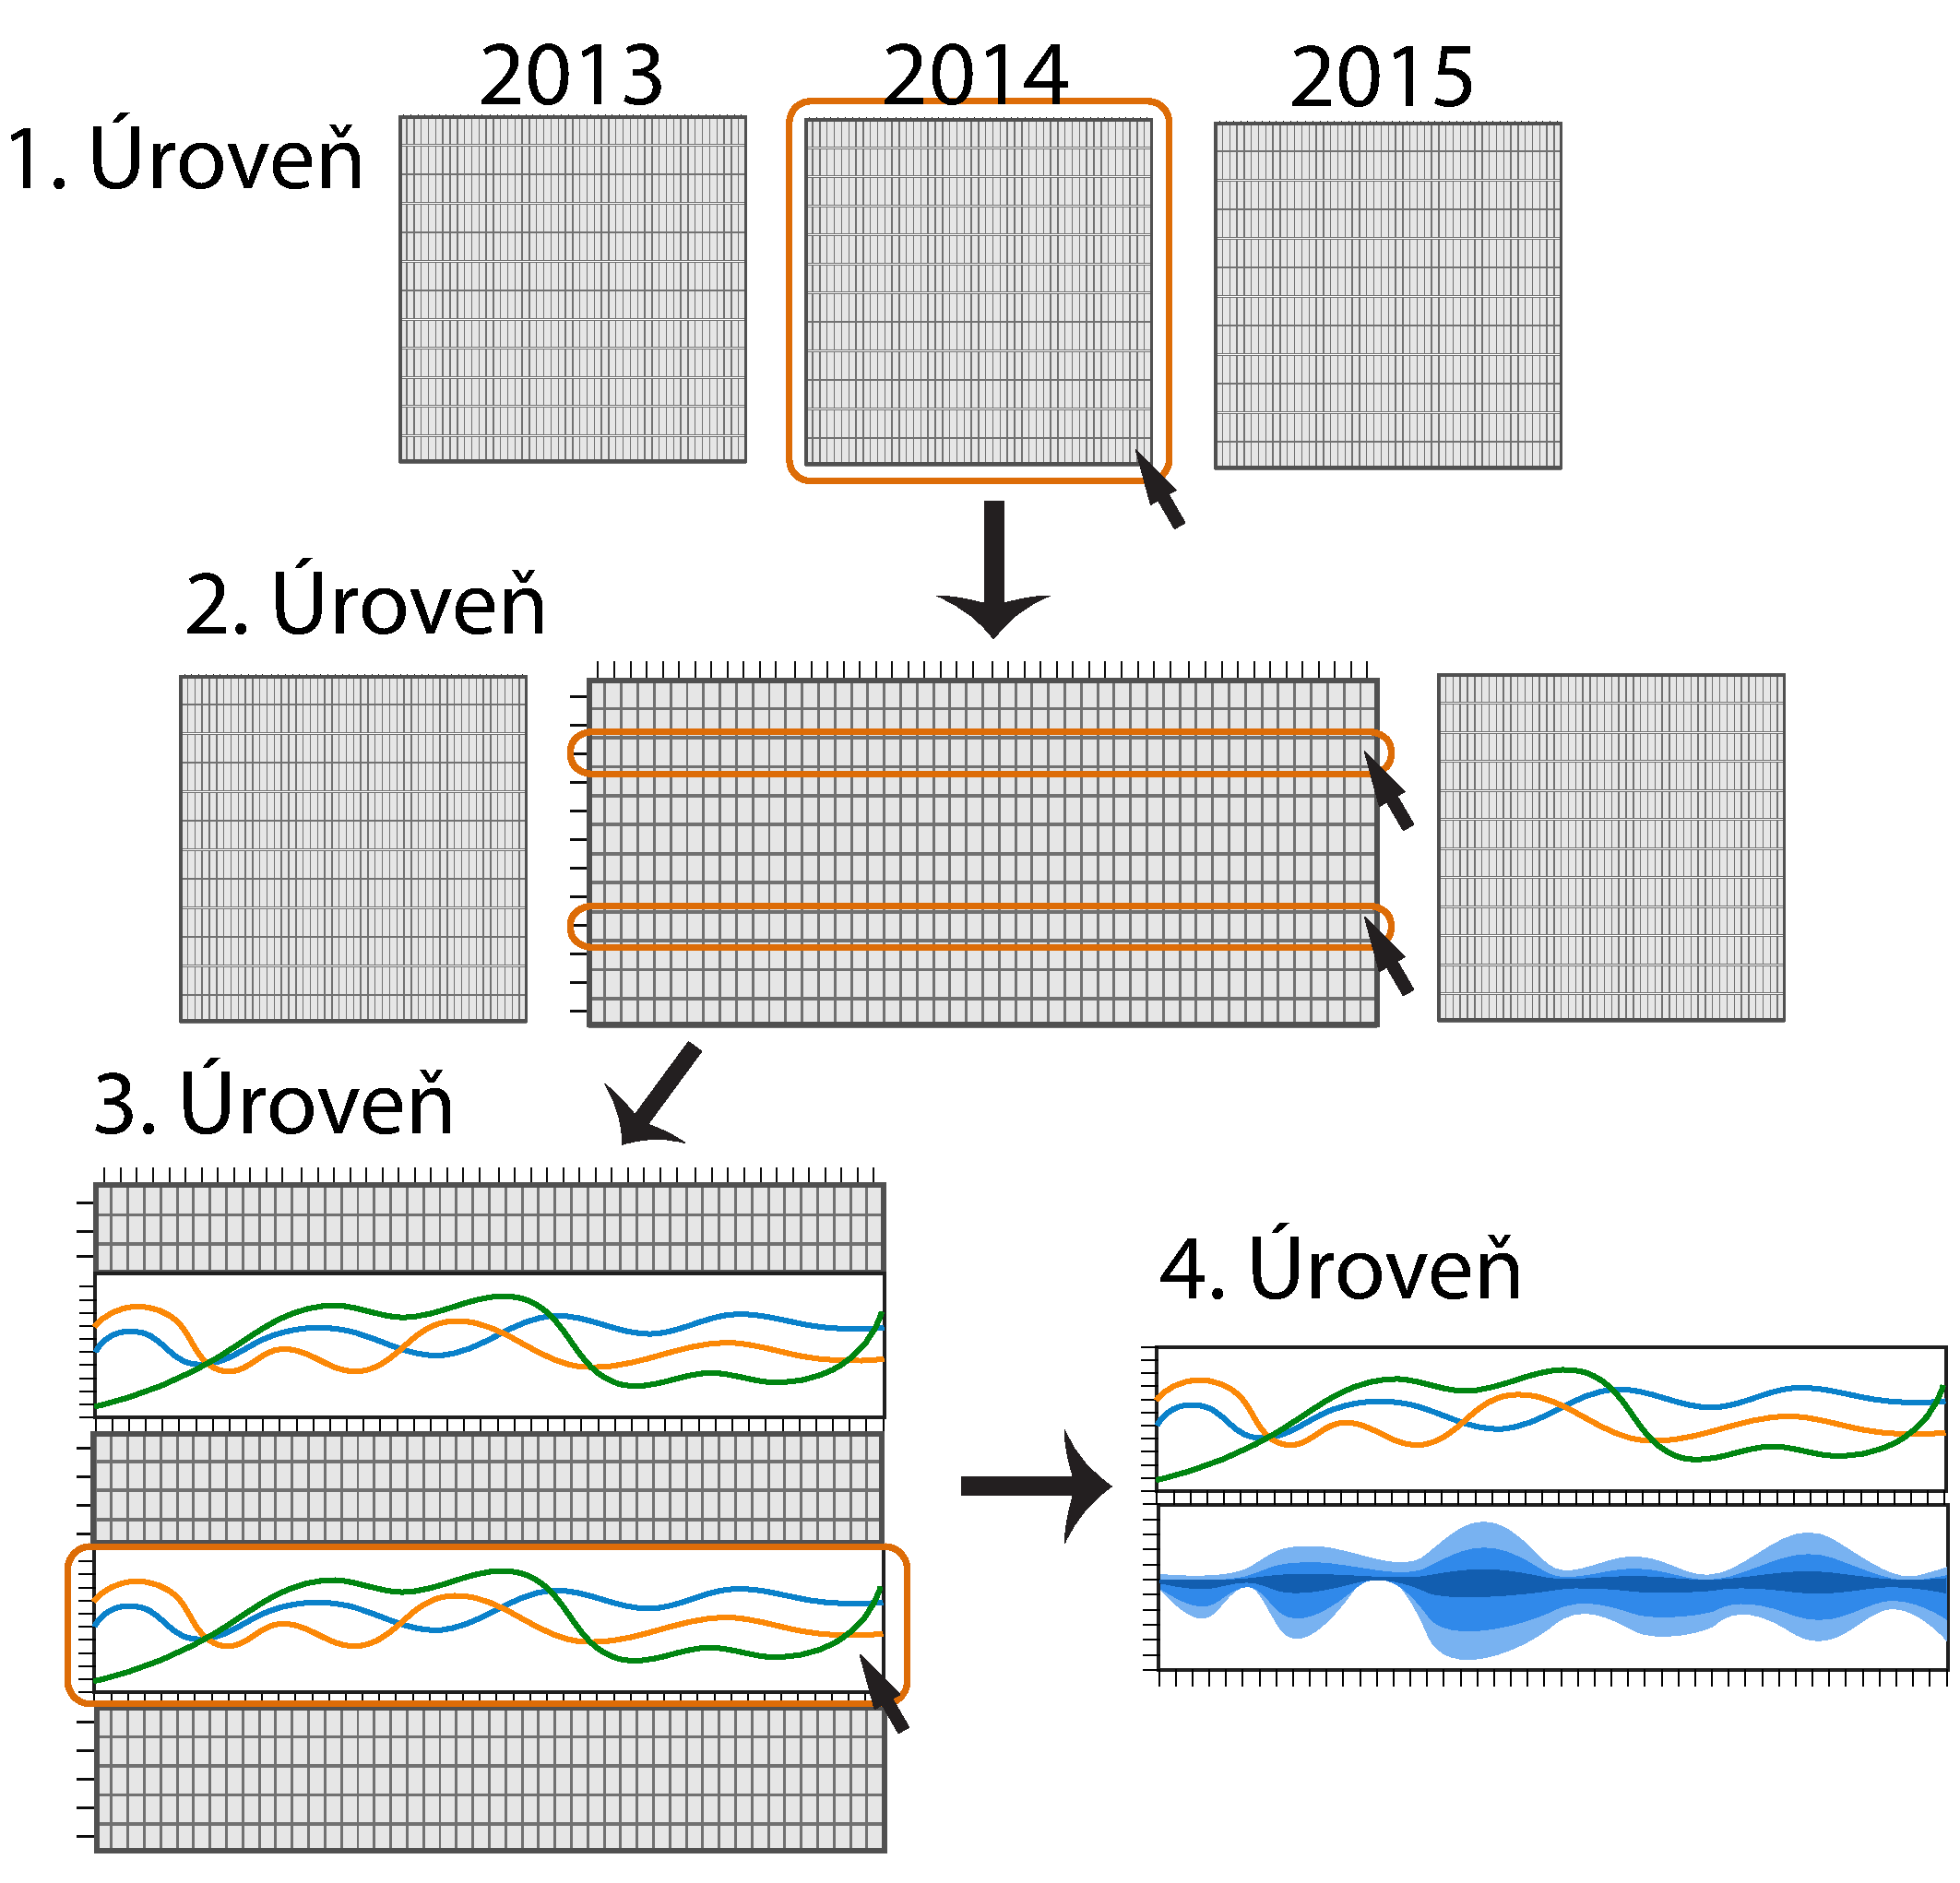
\includegraphics[width = 3.5in]{multilevellayout}
	\caption{Schematické zobrazenie viacúrovňového návrhu rozloženia prvkov vizualizácie}
	\label{fig:multilevellayout}
\end{figure}


\subsection{Plochý návrh rozloženia prvkov}
Pre užívateľa nie je príjemné, keď sa na obrazovke prvky zväčšujú, zmenšujú, posúvajú, objavujú alebo miznú, pretože ... %TODO stráca prehľad alebo čo :D
Preto sme navrhli iný spôsob rozloženia, ktorý tento problém rieši tak, že zobrazí všetky prvky súčasne na jednej úrovni, a teda pojem \textit{úroveň} už nie je potrebný. Spôsob, akým sme umiestnili jednotlivé prvky je schematicky znázornený na obrázku \ref{fig:flatlayout}. Ak potrebujeme vidieť detailnejšie informácie o výkone modelu v mesiaci, tak kliknutím na konkrétny mesiac v prvku \textit{Prehľad}, sa zobrazí \textit{Detail štatistík}, \textit{Distribúcia chýb}, \textit{Detail chýb} pre daný mesiac.

Nevýhodou tohto návrhu je, že nemožno zobraziť viacero prvkov jedného typu súčasne. Z tohto dôvodu nie je možné porovnávať viacero rokov súčasne a preto nie je potrebný komponent \textit{Zjednodušený prehľad}. Zvyšné potrebné porovnávania pre mesiace a distribúciu zaobstará v zníženom, ale dostatočnom detaile, prvok \textit{Prehľad}. 

\begin{figure}
	\centering
	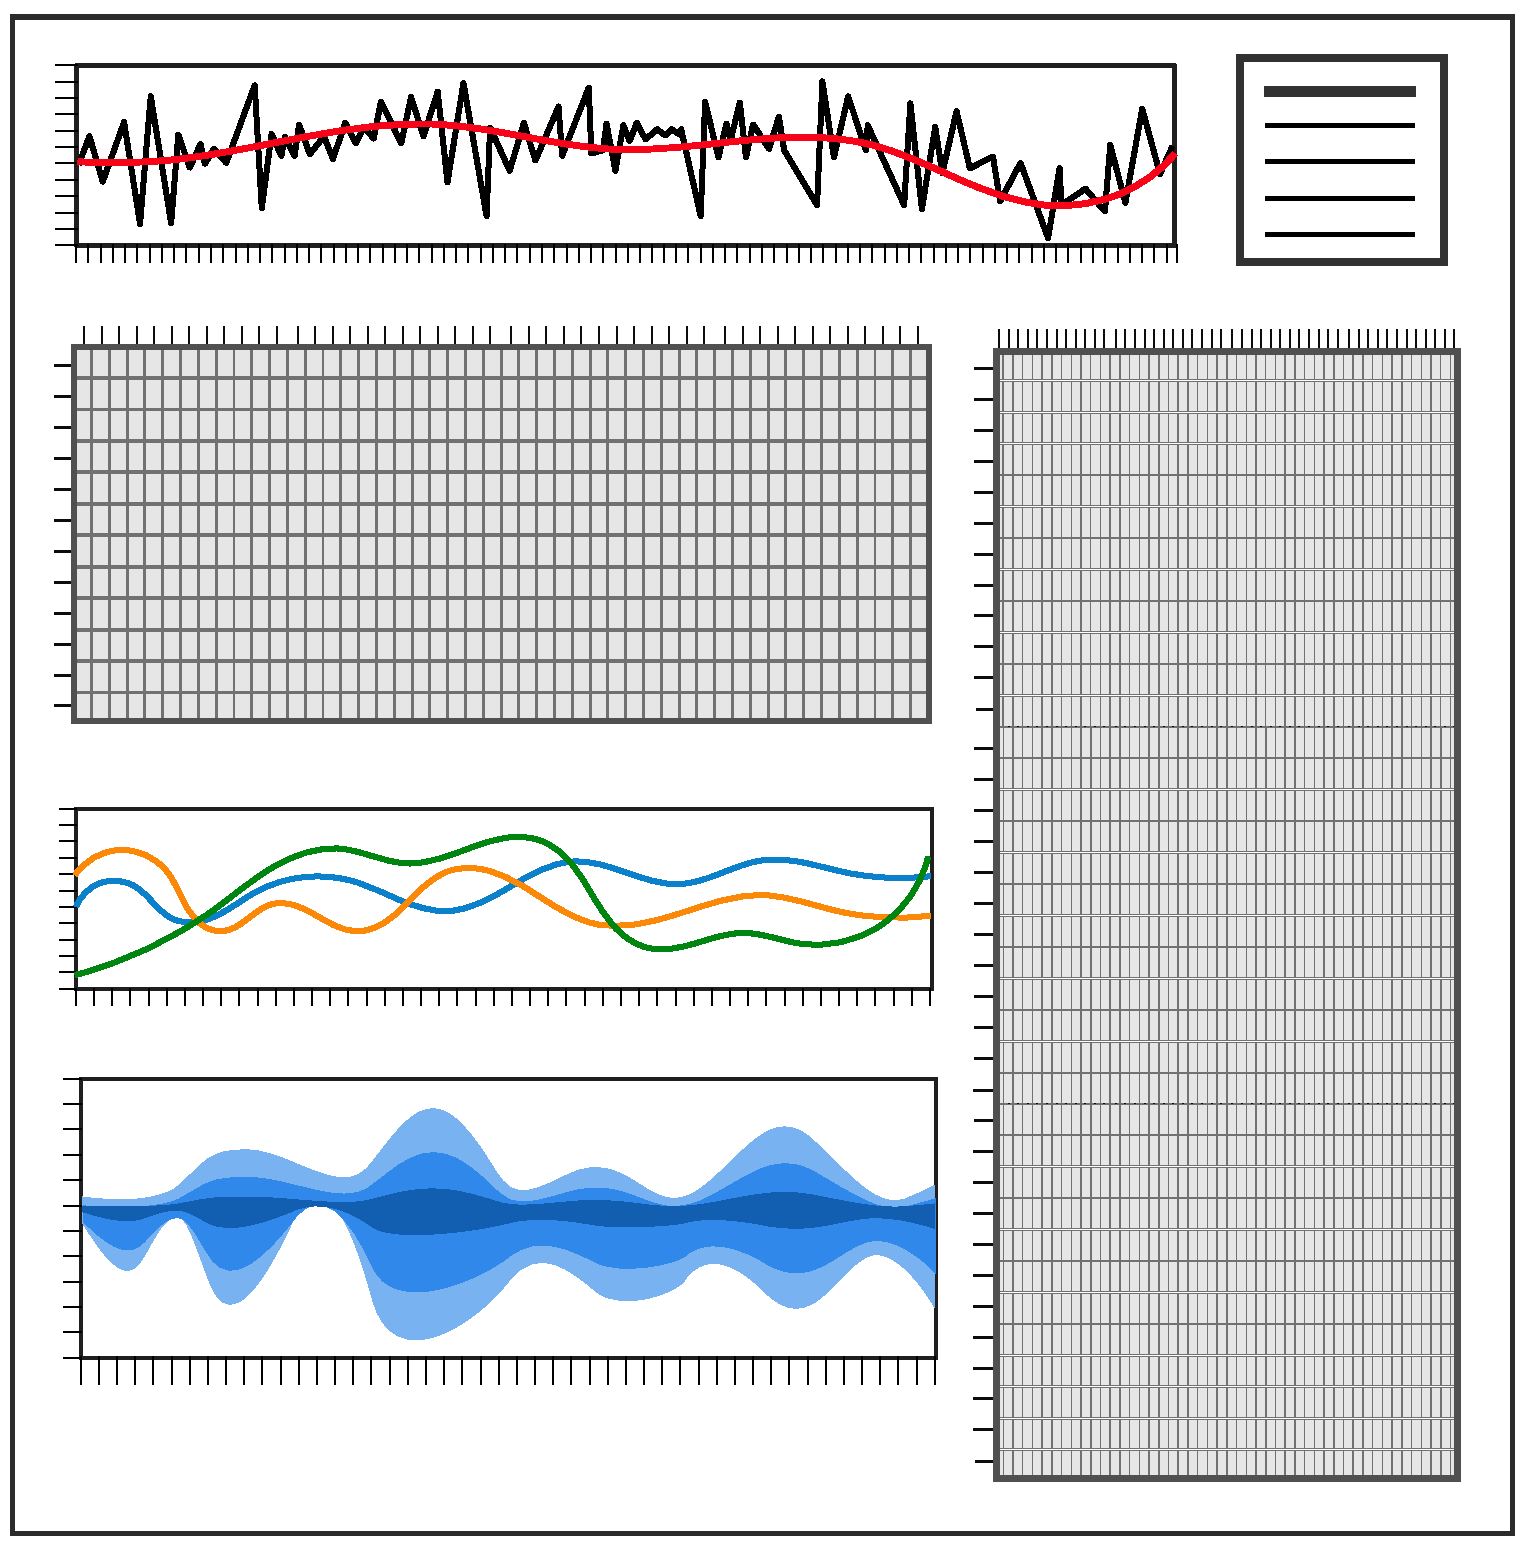
\includegraphics[width = 3.0in]{flatlayout}
	\caption{Schematické zobrazenie plochého návrhu rozloženia prvkov vizualizácie}
	\label{fig:flatlayout}
\end{figure}
